\documentclass[12pt]{article}
    %\usepackage{fullpage}
    \usepackage{epic}
    \usepackage{eepic}
    \usepackage{paralist}
    \usepackage{graphicx}
    \usepackage{caption}
    \usepackage{subcaption}
    \usepackage{enumitem}
    \usepackage{hyperref}
    \usepackage{setspace}
    \doublespacing
    \usepackage{amsmath,amssymb,latexsym,listings}
    \usepackage{algorithm,algorithmic}
    \usepackage{tikz}
    \usepackage{xcolor,colortbl}
    \usepackage{wrapfig}
    
    
    %%%%%%%%%%%%%%%%%%%%%%%%%%%%%%%%%%%%%%%%%%%%%%%%%%%%%%%%%%%%%%%%
    % This is FULLPAGE.STY by H.Partl, Version 2 as of 15 Dec 1988.
    % Document Style Option to fill the paper just like Plain TeX.
    
    \typeout{Style Option FULLPAGE Version 2 as of 15 Dec 1988}
    
    \topmargin 0pt
    \advance \topmargin by -\headheight
    \advance \topmargin by -\headsep
    
    \textheight 8.9in
    
    \oddsidemargin 0pt
    \evensidemargin \oddsidemargin
    \marginparwidth 0.5in
    
    \textwidth 6.5in
    %%%%%%%%%%%%%%%%%%%%%%%%%%%%%%%%%%%%%%%%%%%%%%%%%%%%%%%%%%%%%%%%
    
    \pagestyle{empty}
    \setlength{\oddsidemargin}{0in}
    \setlength{\topmargin}{-0.8in}
    \setlength{\textwidth}{6.8in}
    \setlength{\textheight}{9.5in}
    
    
    \def\ind{\hspace*{0.3in}}
    \def\gap{0.1in}
    \def\bigap{0.25in}
    \newcommand{\Xomit}[1]{}
    
    \DeclareMathOperator*{\argmin}{arg\,min}
    \DeclareMathOperator*{\argmax}{arg\,max}
    
    \begin{document}
    \setlength{\parindent}{0in}
    \addtolength{\parskip}{0.1cm}
    \setlength{\fboxrule}{.5mm}\setlength{\fboxsep}{1.2mm}
    \newlength{\boxlength}\setlength{\boxlength}{\textwidth}
    \addtolength{\boxlength}{-4mm}
    \begin{center}\framebox{\parbox{\boxlength}{{\bf
    CS 4701 \hfill Final Project Report}\\
    Title: \textbf{Studying Modern NBA Positions Using Neural Nets} \hfill Dilip Thiagarajan
    }}
    \end{center}
    \vspace{5mm}
    \section{Introduction}
    Since the its inception to about 2010, the NBA was characterized by teams anchored by tall, strong players standing near the hoop, exemplified by players at center (position) like Wilt Chamberlain, Bill Russell, Kareem Abdul-Jabbar, and Shaquille O'Neal. However, in recent years, the league has been dominated by players on the other end of the height spectrum, being deceptively quick and accurate sharpshooters who extend the floor more widely than before, and teams have had to adjust accordingly by taking out players too slow to keep up. As a result, the center role has dramatically changed, exposing a broad spectrum within the center role, as well as fracturing other traditional roles while combining others.

    As a result, in studying the different archetypes of players using characteristic statistics,  one would find that the traditional split of 5 roles (point guard, shooting guard, small forward, power forward, center) is not an accurate description of the roles the 5 players on the court usually play in today's game, especially for the most prominent players. Take, for example, players like LeBron James or Giannis Antetokounmpo - they are 6'9" and 6'11" in height, respectively, but they don't really play the role of forward or center usually, as would be prescribed traditionally based on their heights. In fact, watching their gameplay, they more closely resemble a point guard rather than any other role, but the traditional point guard doesn't really comprise what they contribute to their team, given how much of the team's success rests on their play. This is just one of several examples where traditional roles doesn't really do the player justice.
    
    In 2010, Muthu Alagappan used this kind of analysis to support his general argument that \textbf{positions don't reflect playing styles}, and are an oversimplification of the true set of roles in basketball. In his study, Alagappan claimed that there were 13 characteristic roles, and supported this using a clustering algorithm with a linear objective. In most further studies aiming to reproduce his results, there have always been about 8-13 characteristic roles that are identified that accurately group a player's playing style with other similar players, using statistics such as points/assists/steals/rebounds per 100 possessions, player efficiency rating, win shares, and more.
    
    While these analyses have been eye-opening in how they discover these natural groupings based on characteristics we can't really quantify, there still seems to be a high magnitude of variance, especially when evaluating a player's performance after a trade or free agency signing given their performance from their previous team. In that sense, I thought it would be interesting to study how fitting these function spaces (over the statistics mentioned above) and looking for a non-linear function that represents these statistics in a lower-dimensional space. As such, I aim to expand on previous studies by examining how autoencoders fit the data, in varying complexities.
    \section{Methods}
    In this section, I describe the methods I used in my analysis of the data. The data I used was all data for NBA players from the 2016-17 season available from Basketball Reference. The data was scraped by formatting the data as a CSV from the website and accordingly downloaded.
    \subsection{Preprocessing}
    The data, when initially scraped, had features such as rank (with respect to certain metrics), player name, and position. I stored the player name as a ways of identifying which row of a matrix of statistics corresponds to which player, and I removed position, as our analysis is predicated on the fact that these positions aren't descriptive. I chose to leave the team as a feature considered because I thought it might uncover relationships between players on the same team, and use that in the representation later on. Finally, if a player changed teams mid-season, I considered their total statistics (i.e. averaged over their performance regardless of team). This gives three sets of data, corresponding to advanced metrics, per-possession metrics, and per-minute (per-36 in the code) metrics. The latter two are similar in the categories they measure, but different in the various biases they have - per-possession favors those who hold the ball less but shoot more, while per-minute favors those who hold the ball more.
    \subsection{Baselines}
    The premise of this problem is dimensionality reduction, and, as mentioned above, past analysis has primarily used linear methods. Thus, as a means of comparison, I choose to examine how a linear dimensionality reduction algorithm arranges the data. Accordingly, I used principal component analysis (PCA) to project the three sets of data to 5, 8, and 13 dimensions. These choices of dimensions, which are used frequently later as well, come from the bounds mentioned above (8-13), and 5 for the number of traditional positions. In that sense, they're not quite arbitrary, but any number above 5 ranging to about 20 would probably be reasonable.

    Additionally, given that we are visualizing the data using t-SNE, we also compare our results after encoding the data with the results of not encoding any of the data, i.e. just running t-SNE on the original data.
    \subsection{Autoencoders}
    \subsection{Structure}
    Autoencoders are a form of dimensionality reduction that leverages the universal approximation power of neural networks. Specifically, autoencoders have the general structure shown below (image from Wikipedia). Given some input $x$, autoencoders try to learn a latent representation $z$ by training two functions $e$ and $d$ such that $(d(e(x)) = x, e(x) = z)$. We refer to the functions $e$ and $d$ as encoder and decoder, and they comprise the left and right half of the autoencoder's structure, respectively.
    \begin{center}
        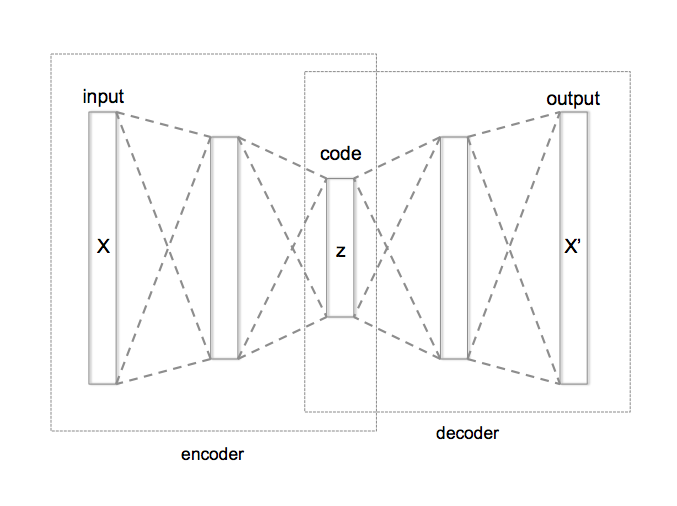
\includegraphics[scale=0.5]{autoencoder-structure}
    \end{center}
    In our study, we'll examine $z$ in dimensions 5, 8, and 13, for the same reasons as mentioned above.
    \subsubsection{Single vs. Multiple Layer Autoencoder}
    While having multiple layers might improve the performance of the net on fitting to a smaller set of data (although it could overfit with higher probability), it's possible that the success of the linear dimensionality reduction techniques is due to their simplicity. As such, I will compare single layer vs. multiple layer autencoders and how they perform on our data.
    \subsection{Implementation}
    The autoencoder classes are implemented in PyTorch, an open-source machine learning package written by Facebook, with a dynamic graph-computation scheme that makes it very easy to implement unique structures like autoencoders.
    \subsection{Training}
    Three single layer autoencoder models were trained separately on the three sets of data, for each representation dimension (5, 8, 13). Then, three multilayer autoencoder models were trained separately as well, with the structure having two hidden layers (13 and 8 dimensions, respectively) between the input and representation layer, and two hidden layers (8 and 13 dimensions, respectively) between the representation and output layer.
    \subsection{Visualization}
    To visualize results in 2-dimensions, the t-SNE algorithm was used. t-SNE is an algorithm that leverages assumptions about the manifold that the data occupies. Simply put, it makes the assumption that the high-dimensional data actually occupies a low-dimensional linear subspace. It is one of the only prominent methods used for visualizing representations learned by a neural net, and is thus the only method I choose to use here for visualizing the data.
    \subsection{Evaluation}
    Quantifying how good the roles are in this problem is difficult given the unsupervised nature of the overarching problem. As a result, I choose to look at the 5 closest neighbors for the points and evaluate them ad-hoc, based on my own judgement. I look at the closest neighbors after both the choice of embedding and t-SNE. For convenience, the results are displayed in the notebook, and not here.
    \subsection{Variational Approach}
    While I mentioned the variational approach in my proposal, I decided to leave it out, as the results I was getting from the variational approach were pretty much identical to the discriminative approach.
    \section{Results}
    \subsection{T-SNE}
    Below is the visualization for the data after running the t-SNE algorithm with 2 components.
    \begin{center}
        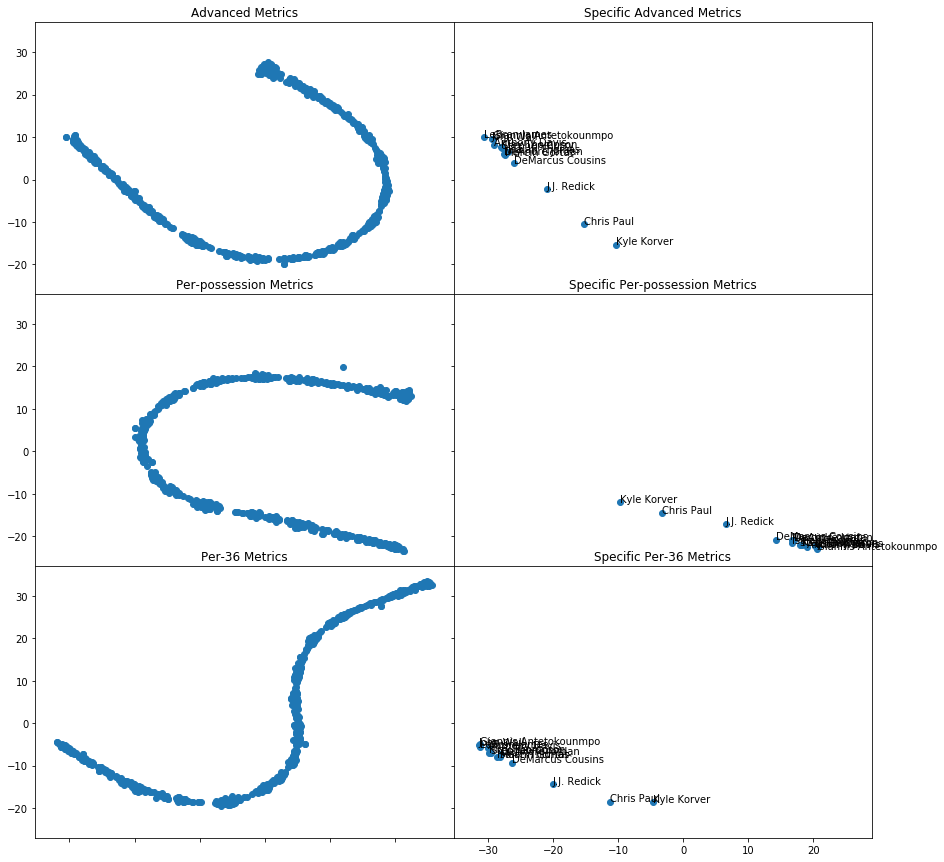
\includegraphics[scale=0.5]{images/only-tsne}
    \end{center}
    \subsection{PCA and T-SNE}
    Below is the visualization for the data after PCA with 5 components and running the t-SNE algorithm with 2 components.
    \begin{center}
        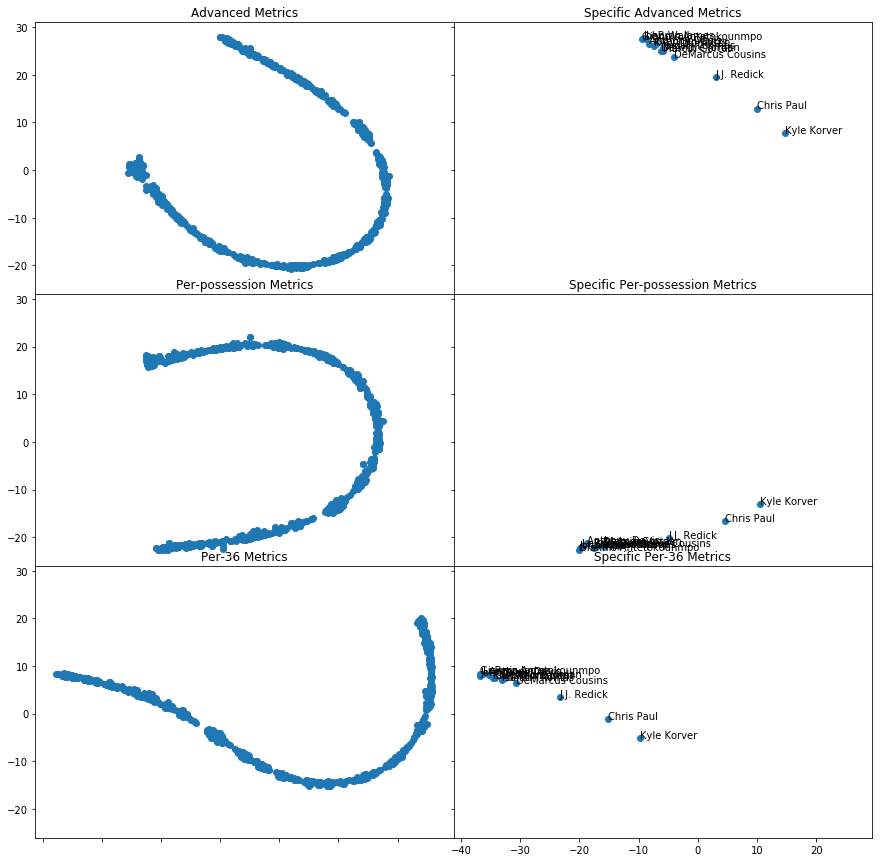
\includegraphics[scale=0.5]{images/pca-5}
    \end{center}
    Below is the visualization for the data after PCA with 8 components and running the t-SNE algorithm with 2 components.
    \begin{center}
        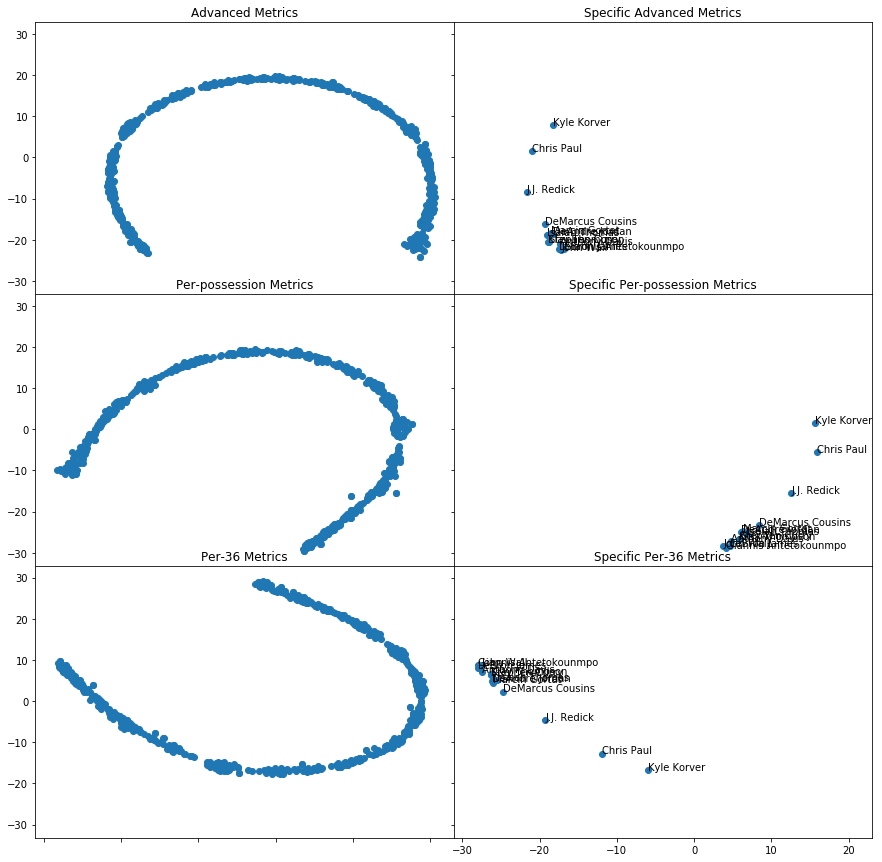
\includegraphics[scale=0.5]{images/pca-8}
    \end{center}
    Below is the visualization for the data after PCA with 13 components and running the t-SNE algorithm with 2 components.
    \begin{center}
        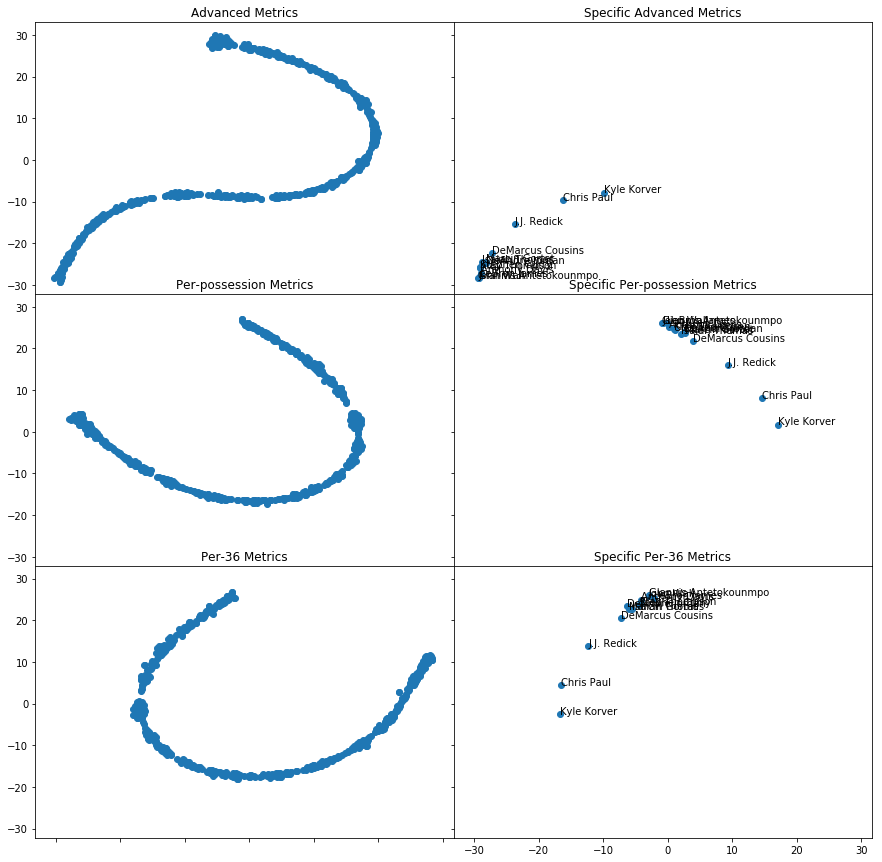
\includegraphics[scale=0.5]{images/pca-13}
    \end{center}
    \subsection{Single Layer Autoencoder and T-SNE}
    Below is the visualization for the data after training a single-layer autoencoder with 5 components and running the t-SNE algorithm with 2 components.
    \begin{center}
        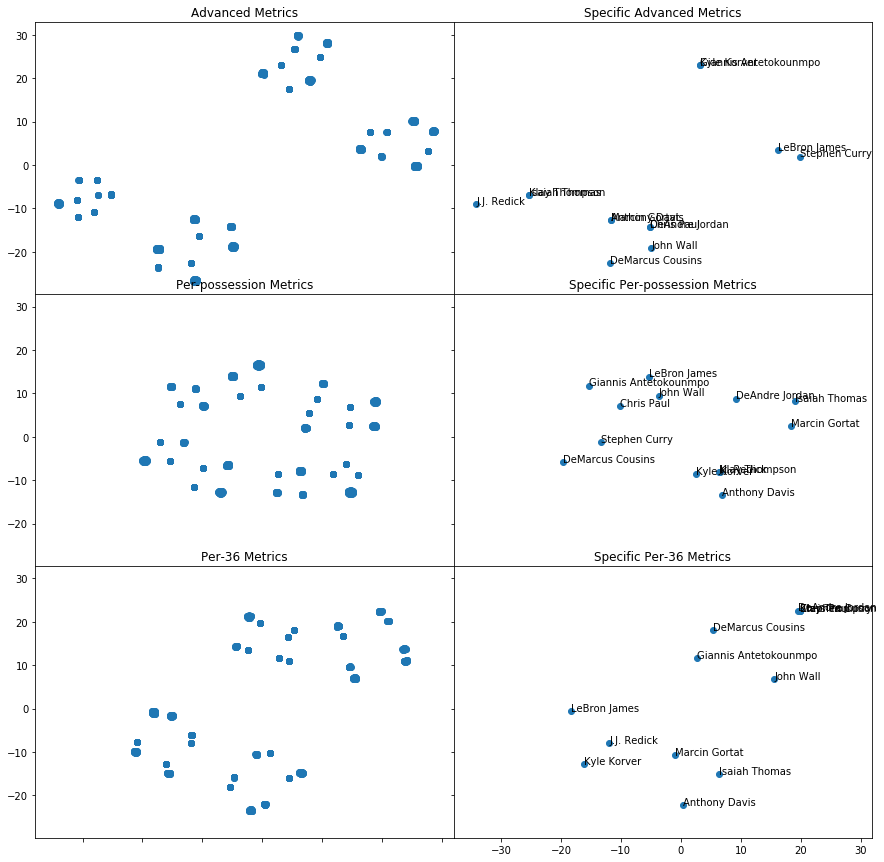
\includegraphics[scale=0.5]{images/single-layer-5}
    \end{center}
    Below is the visualization for the data after training a single-layer autoencoder with 8 components and running the t-SNE algorithm with 2 components.
    \begin{center}
        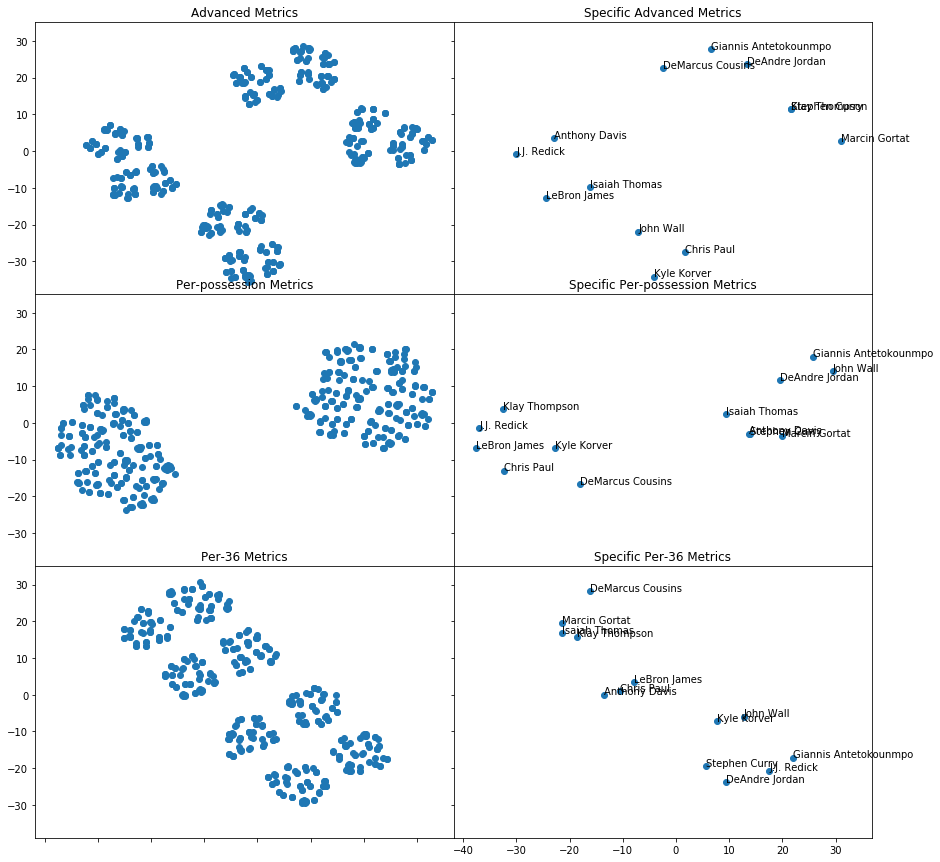
\includegraphics[scale=0.5]{images/single-layer-8}
    \end{center}
    Below is the visualization for the data after training a single-layer autoencoder with 13 components and running the t-SNE algorithm with 2 components.
    \begin{center}
        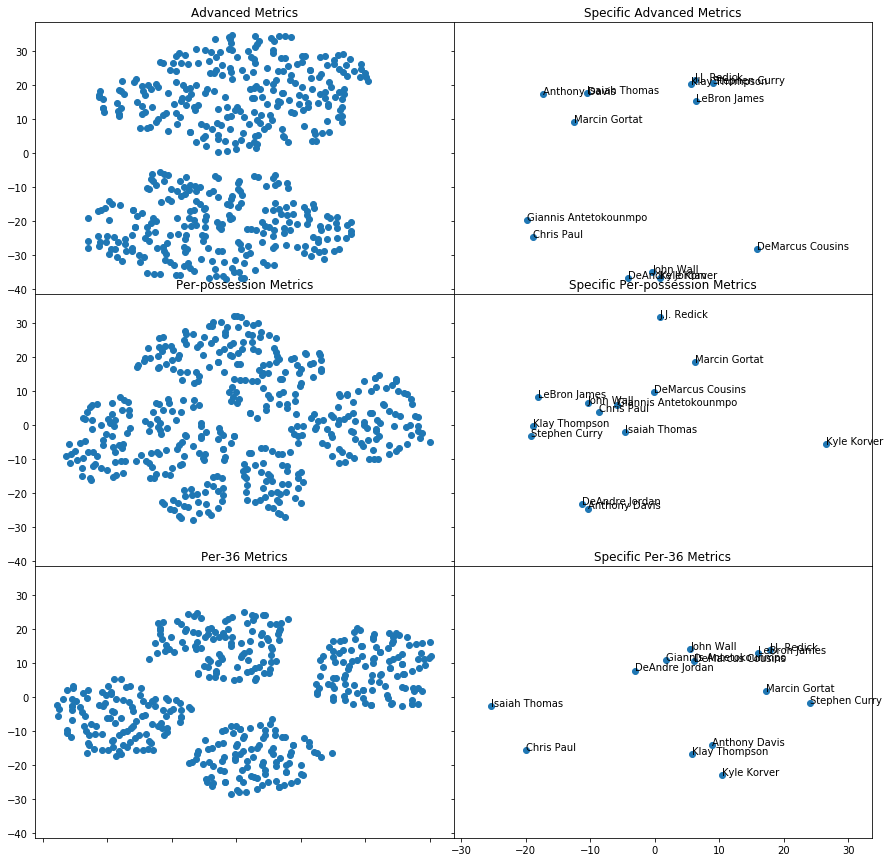
\includegraphics[scale=0.5]{images/single-layer-13}
    \end{center}
    \subsection{Multilayer Autoencoder and T-SNE}
    Below is the visualization for the data after training a multi-layer autoencoder as specified above with 5 components and running the t-SNE algorithm with 2 components.
    \begin{center}
        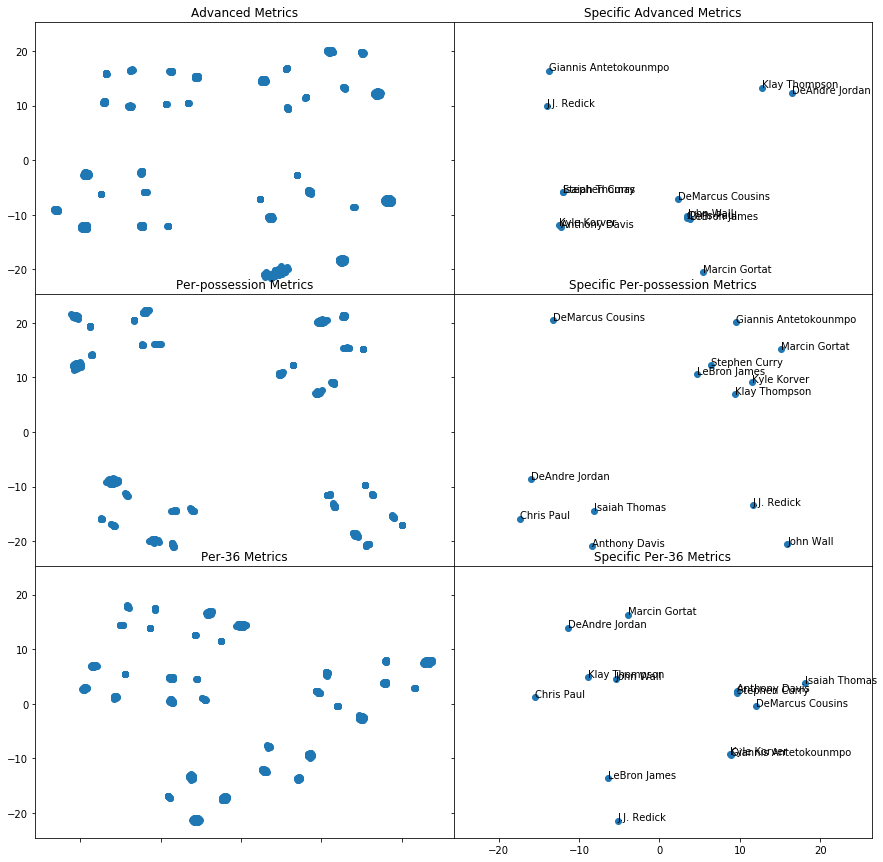
\includegraphics[scale=0.5]{images/multi-layer}
    \end{center}
    \section{Discussion}
    One thing that was particularly interesting throughout this study was that as the complexity of the overall model increased (e.g. from just t-SNE to PCA+t-SNE to single-layer autoencoder+t-SNE to multi-layer autoencoder+t-SNE), the points seemed to clump into well-formed clusters. This was an interesting thing to observe given that the performance of the model didn't really seem to improve consistently, based on examining the 5 closest neighbors. However, upon examining the visualizations, we do see between 5-13 clusters usually, depending on what clustering objective is chosen, which might indicate some other similarity in the players that's much more subtle and harder to identify.

    However, this phenomenon actually reversed when increasing the representation size of the single-layer autoencoder. Given this trend, I imagine that the same thing would be observed when increasing the representation size of the multi-layer autoencoder. This is a bit unexpected, given that adding more dimensions to the representation should theoretically allow the model to separate points more easily,but it seems that it's fitting more towards how the original data looks like, i.e. visualizing them without any sort of embedding, including t-SNE. One thing that might reverse this phenomenon would be to constrain the loss function more tightly - we used the constraint that the input and output layers should be as close as possible. Maybe constraining that symmetric layers should be as close as possible would achieve the desired effect of more separation as representation size increases.

    Another thing that was interesting was how the encoding of the metrics never lost the biases mentioned previously. Specifically, per-possession encodings still seemd to group players with high usage percentages (i.e. held the ball a lot), while per-36 metrics group players who shot the ball more often than not, even when encoding using more complex models. In a sense, this is proper, given that these biases are inherent to the data, and losing sight of this information would be an indication that the subspace the data occupies isn't being characterized properly by the neural model.

    One thing that could have helped in all aspects of this study would be to include more data. I was skeptical in doing this given how the change in rules and playstyle often changes the role players fill in the game, but it definitely would be reasonable to include more than just 1 years worth of data. To do so, each player's statistics for 1 year could be considered separately, instead of combined, which not only would allow for more data, but would allow the visualizations to signify any progression the players make from 1 role (grouping in the visualization) to another.

    Another thing that could have helped was to more closely validate each of the models based on finer details such as learning rate, activation functions, dropout probability, optimizer, and more. However, it seemed that this wouldn't have had much of an effect, given that the loss after training was pretty similar for the same types of models.
    \section{Conclusion}
    In this study, we've examined using non-linear function spaces to fit subspaces of the data space summarizing the 2016-17 NBA season for each player. While the results were interesting, it seems that non-linear function spaces aren't very good at summarizing player roles. However, additional constraints on the learning algorithm might have reduced the complexity of the model's learned function, so further work expanding on that would probably find something more significant with respect to player similarity and role separation.
    \section{Appendix}
    The code for this study and relevant images can be found \href{https://github.com/dthiagarajan/4701_project}{here}. The link is a Github account repo (dthiagarajan is the account, 4701 project is the repo).
    \end{document}
    